\begin{wrapfigure}[6]{r}[0pt]{100mm}
	\centering
    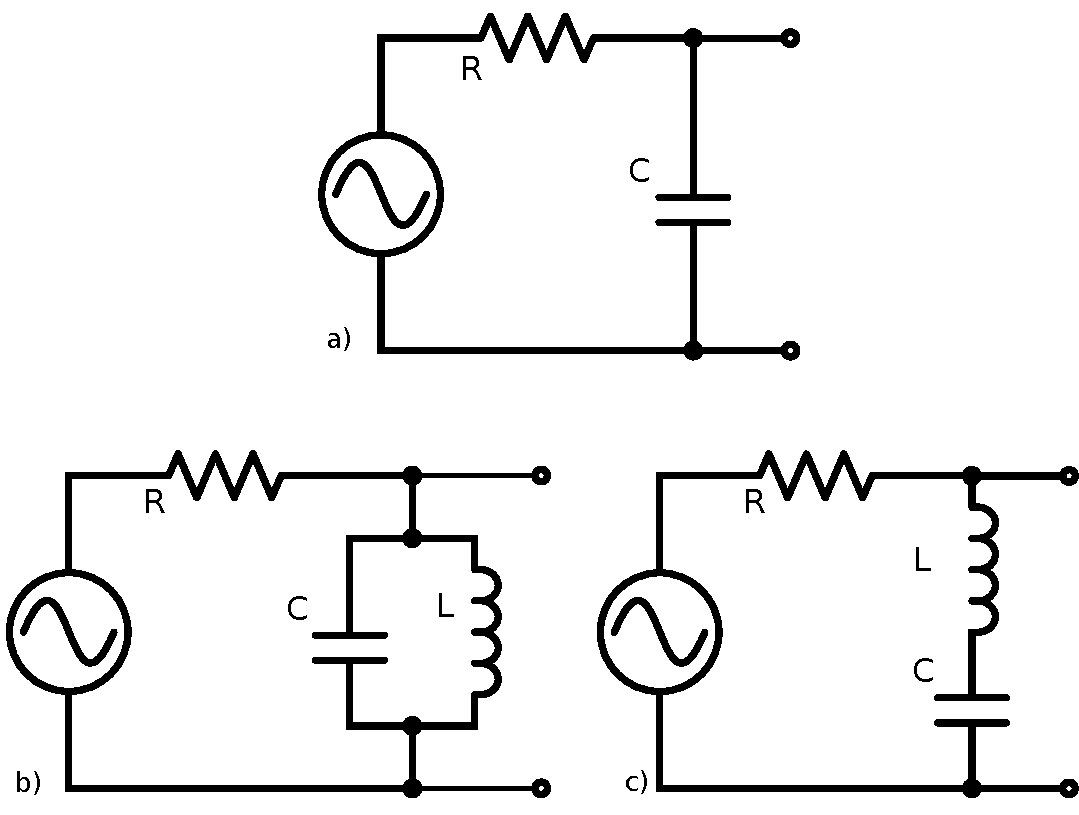
\includegraphics[width=0.40\textwidth]{circuiti2.pdf}
    \caption{Schema dei circuiti utilizzati: a) filtro passa basso;\\ b) filtro passa banda; c) filtro a reiezione di banda}
    \label{fig:circuito}
\end{wrapfigure}

Mediante l'oscilloscopio, verificare la funzione di trasferimento per filtri passa basso, passa banda e reiezione di banda.
\section{Strumenti}

$\bullet \quad$Oscilloscopio \\
$\bullet \quad$Cablaggio\\
$\bullet \quad$Breadboard\\
$\bullet \quad$Generatore di forme d'onda\\
$\bullet \quad$Multimetro digitale\\
$\bullet \quad$Decadi di resistenze,\\
\phantom{xxx}capacitori e induttanze\\
